% Uebung Nr. 3 Zeigerdiagramm nach Brinkmeyer
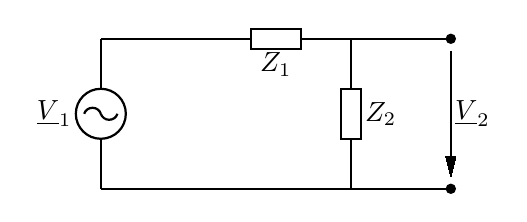
\begin{tikzpicture}[scale=2.54]%
% dpic version 2024.01.01 option -g for TikZ and PGF 1.01
\ifx\dpiclw\undefined\newdimen\dpiclw\fi
\global\def\dpicdraw{\draw[line width=\dpiclw]}
\global\def\dpicstop{;}
\dpiclw=0.8bp
\dpiclw=0.8bp
\dpicdraw (0,0)
 --(0,-0.25)\dpicstop
\dpicdraw (0,-0.375) circle (0.049213in)\dpicstop
\dpicdraw (-0,-0.375)
 ..controls (-0.005978,-0.357065) and (-0.022762,-0.344968)
 ..(-0.041667,-0.344968)
 ..controls (-0.060571,-0.344968) and (-0.077355,-0.357065)
 ..(-0.083333,-0.375)\dpicstop
\dpicdraw (0,-0.375)
 ..controls (0.005978,-0.392935) and (0.022762,-0.405032)
 ..(0.041667,-0.405032)
 ..controls (0.060571,-0.405032) and (0.077355,-0.392935)
 ..(0.083333,-0.375)\dpicstop
\dpicdraw (0,-0.5)
 --(0,-0.75)\dpicstop
\draw (-0.125,-0.375) node[left=-2bp]{$ \underline{V}_1$};
\dpicdraw (0,0)
 --(0.5,0)\dpicstop
\dpicdraw (0.5,0)
 --(0.75,0)\dpicstop
\dpicdraw (1,0)
 --(1,0.05)
 --(0.75,0.05)
 --(0.75,-0.05)
 --(1,-0.05)
 --(1,0)\dpicstop
\dpicdraw (1,0)
 --(1.25,0)\dpicstop
\draw (0.875,-0.05) node[below=-2bp]{$ Z_1$};
\dpicdraw (1.25,0)
 --(1.25,-0.25)\dpicstop
\dpicdraw (1.25,-0.5)
 --(1.3,-0.5)
 --(1.3,-0.25)
 --(1.2,-0.25)
 --(1.2,-0.5)
 --(1.25,-0.5)\dpicstop
\dpicdraw (1.25,-0.5)
 --(1.25,-0.75)\dpicstop
\draw (1.3,-0.375) node[right=-2bp]{$ Z_2$};
\dpicdraw (1.25,0)
 --(1.75,0)\dpicstop
\dpicdraw[fill=black](1.75,0) circle (0.007874in)\dpicstop
\dpicdraw[fill=black](1.75,-0.75) circle (0.007874in)\dpicstop
\filldraw[line width=0bp](1.725,-0.59)
 --(1.75,-0.69)
 --(1.775,-0.59) --cycle\dpicstop
\dpicdraw (1.75,-0.06)
 --(1.75,-0.667094)\dpicstop
\draw (1.75,-0.375) node[right=-2bp]{$ \underline{V}_2$};
\dpicdraw (1.75,-0.75)
 --(0,-0.75)\dpicstop
\end{tikzpicture}%
